% Created 2017-02-20 Mon 21:40
% Intended LaTeX compiler: pdflatex
\documentclass[bigger]{beamer}
\usepackage[utf8]{inputenc}
\usepackage[T1]{fontenc}
\usepackage{graphicx}
\usepackage{grffile}
\usepackage{longtable}
\usepackage{wrapfig}
\usepackage{rotating}
\usepackage[normalem]{ulem}
\usepackage{amsmath}
\usepackage{textcomp}
\usepackage{amssymb}
\usepackage{capt-of}
\usepackage{hyperref}
\mode<beamer>{\usetheme{Singapore}}
\mode<beamer>{\usecolortheme{wolverine}}
\mode<beamer>{\usefonttheme{structurebold}}
\author{Kevin Nolan}
\date{\today}
\title{Thesis proposal}
\hypersetup{
 pdfauthor={Kevin Nolan},
 pdftitle={Thesis proposal},
 pdfkeywords={},
 pdfsubject={},
 pdfcreator={Emacs 26.0.50.1 (Org mode 9.0.4)}, 
 pdflang={English}}
\begin{document}

\maketitle
\tableofcontents



\section{Introduction}
\label{sec:org74a5974}
\subsection{A simple slide}
\label{sec:orga8d710e}
This slide consists of some text with a number of bullet points:

\begin{itemize}
\item the first, very \textbf{important}, point!
\item the previous point shows the use of the special markup which
translates to the Beamer specific \emph{alert} command for highlighting
text.
\end{itemize}


The above list could be numbered or any other type of list and may
include sub-lists.

\subsection{A more complex slide}
\label{sec:org3eb832f}
This slide illustrates the use of Beamer blocks.  The following text,
with its own headline, is displayed in a block:
\subsubsection{Org mode increases productivity\hfill{}\textsc{B\_theorem}}
\label{sec:org0d29f12}
\begin{itemize}
\item org mode means not having to remember \LaTeX{} commands.
\item it is based on ascii text which is inherently portable.
\item Emacs!
\end{itemize}

\hfill \(\qed\)

\subsection{Two columns}
\label{sec:orgb1d8017}

\subsubsection{A block\hfill{}\textsc{B\_ignoreheading:BMCOL}}
\label{sec:org85e9ee4}
\begin{itemize}
\item this slide consists of two columns
\item the first (left) column has no heading and consists of text
\item the second (right) column has an image and is enclosed in an
\textbf{example} block
\end{itemize}

\subsubsection{A screenshot\hfill{}\textsc{BMCOL:B\_example}}
\label{sec:org36563c4}
\begin{center}
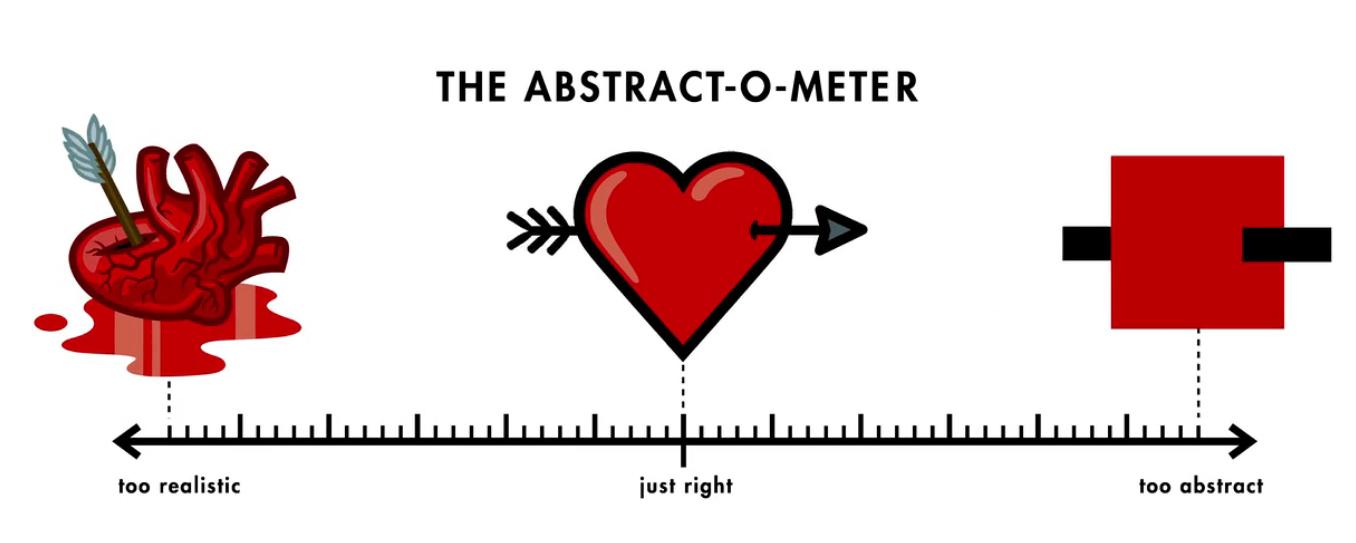
\includegraphics[width=.9\linewidth]{./screenshots/abstract-o-meter.png}
\end{center}

\section{How??}
\label{sec:org689c4ed}
\subsection{A simple slide}
\label{sec:orgc7d98dd}
This slide consists of some text with a number of bullet points:

\begin{itemize}
\item the first, very \textbf{important}, point!
\item the previous point shows the use of the special markup which
translates to the Beamer specific \emph{alert} command for highlighting
text.
\end{itemize}


The above list could be numbered or any other type of list and may
include sub-lists.

\subsection{A more complex slide}
\label{sec:orgf87c157}
This slide illustrates the use of Beamer blocks.  The following text,
with its own headline, is displayed in a block:
\subsubsection{Org mode increases productivity\hfill{}\textsc{B\_theorem}}
\label{sec:org0fa1d1a}
\begin{itemize}
\item org mode means not having to remember \LaTeX{} commands.
\item it is based on ascii text which is inherently portable.
\item Emacs!
\end{itemize}

\hfill \(\qed\)

\subsection{Two columns}
\label{sec:org9c36a99}

\subsubsection{A block\hfill{}\textsc{B\_ignoreheading:BMCOL}}
\label{sec:orgd060934}
\begin{itemize}
\item this slide consists of two columns
\item the first (left) column has no heading and consists of text
\item the second (right) column has an image and is enclosed in an
\textbf{example} block
\end{itemize}

\subsubsection{A screenshot\hfill{}\textsc{BMCOL:B\_example}}
\label{sec:org778000b}
\begin{center}
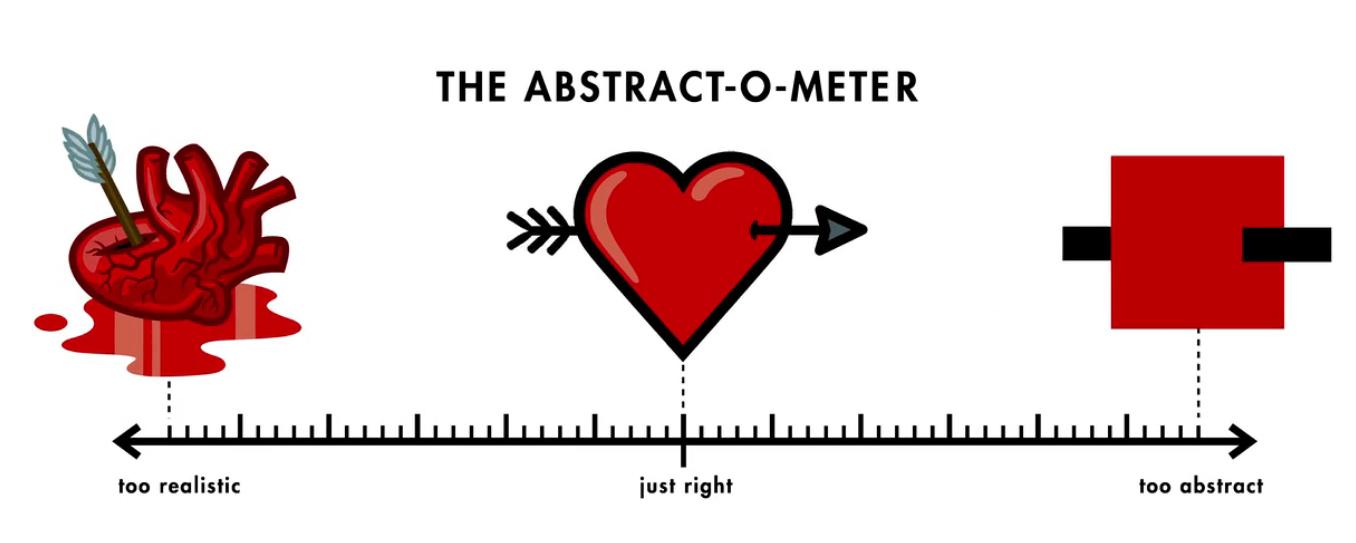
\includegraphics[width=.9\linewidth]{./screenshots/abstract-o-meter.png}
\end{center}
\end{document}
